% This file: 			Prelim. draft for Heckman to see progress
% Contributors: 		Pietro Biroli, Daniela Del Boca, Linor Kiknadze, 
%					Yu Kyung Koh, Sylvi Kuperman, Sidharth Moktan, 
%					Chiara Pronzato, Nirali Trevedi, Anna Ziff
% Original date: 		10/10/16
% Project: 			Reggio Evaluation

\documentclass[12pt]{article}
\usepackage[top=1in, bottom=1in, left=1in, right=1in]{geometry}
\parindent 22pt

\usepackage{adjustbox}
\usepackage{amsmath}
\usepackage{amssymb}
\usepackage{array}
\usepackage{booktabs}
\usepackage{datetime}
\usepackage{fancyhdr}
\usepackage{float}
\usepackage{graphicx}
\usepackage[colorlinks=true,linkcolor=blue,urlcolor=blue,anchorcolor=blue,citecolor=blue]{hyperref}
\usepackage{lscape}
\usepackage{multirow}
\usepackage{natbib}
\usepackage{setspace}
\usepackage{tabularx}
\usepackage[colorinlistoftodos,linecolor=black]{todonotes}
\usepackage{appendix}
\usepackage{pgffor}
\usepackage{caption} 
\usepackage{threeparttable}
\captionsetup[table]{skip=3pt}

\settimeformat{hhmmsstime}

\newcolumntype{L}[1]{>{\raggedright\arraybackslash}p{#1}}
\newcolumntype{C}[1]{>{\centering\arraybackslash}p{#1}}
\newcolumntype{R}[1]{>{\raggedleft\arraybackslash}p{#1}}


\usepackage{sectsty}
\sectionfont{\fontsize{12}{12}\selectfont}

\begin{document}

\title{\normalsize \textbf{Evaluation of the Reggio Approach} \\ \normalsize Draft}
\author{\normalsize Reggio Team}
\date{\normalsize Original version: October 3, 2016 \\ Current version: \today}
\maketitle

\doublespacing

This draft presents (i) a brief description of the data, (ii) a simple analysis comparing individuals who attended the Reggio Emilia municipal schools to individuals in Reggio Emilia who did not attend any preschool, and (iii) a discussion of selection into preschool on observed characteristics. 

\section{Data}
\label{sec:data}

The sample was collected from the population of individuals in Reggio Emilia, Parma, and Padova who were born in the year ranges of the five cohorts.  These individuals were collected from the population registries in each of the cities. The sample was then restricted to those individuals living in the same city in which they were raised. All cohorts except the youngest one were restricted to individuals who are Italian citizens. In contrast, the youngest cohort includes an oversampling of immigrant children. The sample from Reggio Emilia, across all cohorts, includes an oversampling of those who attended municipal schools, as this is considered the treatment.

Of the reference sample, 7,109 individuals were randomly selected. Of these, 4,019 completed interviews, resulting in a response rate of 56.5\%. Figure~\ref{fig:sample} presents an overview of the sample highlighting those who attended a Reggio Approach preschool. Table~\ref{tab:sample} provides a detailed tabulation of the sample by city, cohort, and school type.

\begin{figure}[H]
\begin{center}
\caption{The Sample by City and Cohort}\label{fig:sample}
	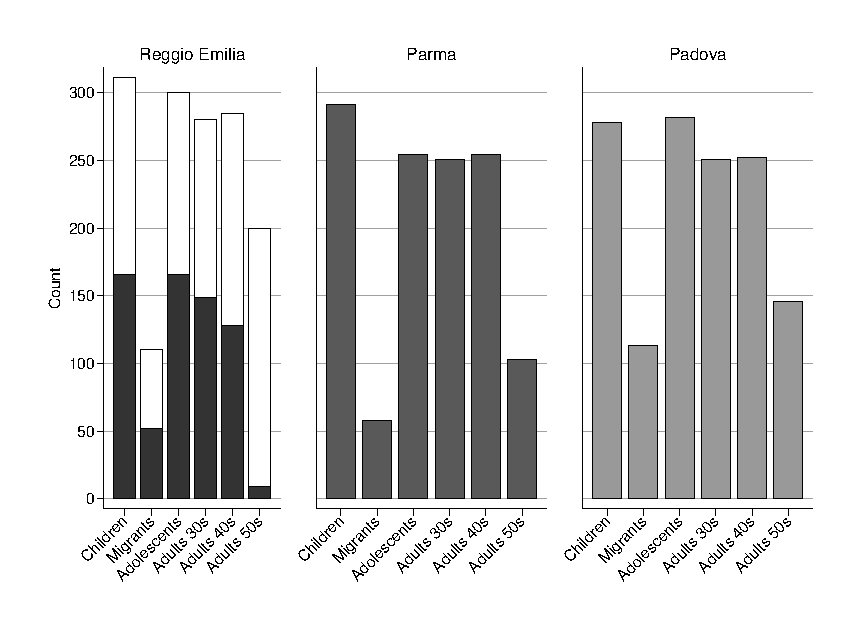
\includegraphics[width=.9\textwidth]{output/sample.eps}
\end{center}
\raggedright
Note: This figure displays the number of individuals by cohort and city. The bars for Reggio Emilia differentiate between those who attended municipal preschool (black bars) and those who did not (white bars). 
\end{figure}

\begin{table}[H]
\centering
\scalebox{0.7}{
\begin{threeparttable}
	\caption{The Sample by Cohort, City, and School Type}\label{tab:sample}
	\begin{tabular}{l*{15}{c}}
\toprule
            &\mc{5}{c}{Reggio Emilia: 1,471}   &     \mc{5}{c}{ Parma: 1,198}       &      \mc{5}{c}{Padova: 1,305}      \\
           \cmidrule(lr){2-6} \cmidrule(lr){7-11} \cmidrule(lr){12-16} 
      &        None&       Muni.&       State&      Relig.&       Priv.&        None&       Muni.&       State&      Relig.&       Priv.&        None&       Muni.&       State&      Relig.&       Priv.\\
\midrule
Children    &           2&         166&          45&          92&           5&           6&         154&          43&        77&           9&           2&          82&          40&         141&          12\\
Migrants    &           4&          52&          37&          14&           1&           4&          35&          10&          	3&           6&           5&          36&          47&          23&           1\\
Adolescents &           7&         166&          22&          96&           6&           4&         116&          43&     82&           6&           1&          93&          47&         131&           6\\
Adults 30    &          57&         149&          31&          40&           1&          44&          98&          51&        50&          5&       47&         35&         26&            140&    1 \\
Adults 40    &          80&         128&          17&          52&           5&         116&          52&          26&       55&          1&        75&      27 &            24&            123&   \\
Adults 50    &         147&           9&          10&          28&           2&          72&          12&           7&          11&            &        57&      11 &           2 &           68&    2 \\
\midrule
	       &         297&         670&         162&         322&          20&         246&         467&   180&    278&          27&      187&      284 &            186&        626& 22  \\
\bottomrule
\end{tabular}


\begin{tablenotes}
Note: This table shows the sample size by city, cohort, and school type. These numbers do not include individuals with an unidentified preschool type. In the whole sample, there are 45 individuals with unidentified preschool type. None: no preschool; Muni.: municipal preschool;  State: state preschool; Relig.: religious preschool; Priv.: private preschool.
\end{tablenotes}
\end{threeparttable}
}
\end{table}

The structure of the cohorts allows us to study the effects of the Reggio Approach at different points throughout the life cycle. The youngest cohort of children were interviewed when they entered primary school, the adolescent cohort when they ended compulsory schooling, and the adult cohorts capture different points of engagement in the labor market and familial decisions. This cohort structure also allows us to evaluate the Reggio Approach compared to the alternative early childhood experiences as they evolved over time.

Separate questionnaires were administered to the children, adolescents, and adults, as well as to the caregivers of the children and adolescents. The questionnaires included items about early childhood experiences, family structure, education, interaction with other ethnicities, and measures cognitive and social-emotional skills. The questionnaires for adults additionally included items about occupation, income, and life satisfaction. 

\section{Basic Analysis}
\label{sec:methodology}

We present a basic specification of OLS to estimate the effect on an outcome of interest, $Y$, of the Reggio Approach compared to not attending preschool at all. For this abbreviated analysis, we restrict to individuals from Reggio Emilia who either attended a Reggio Approach preschool or did not attend any preschool (across all cohorts, $N = 967$).

For individual $i$ in Reggio Emilia, let $\mu_i$ indicate whether that individual attended a Reggio Approach preschool. We select a vector, $\bm{X}_i$, of five baseline control variables with the lowest BIC to account for family background.\footnote{These variables are: \color{maroon}{forthcoming}} We estimate $\beta_1$ in the simple model

\begin{equation}
	Y_i = \beta_0 + \beta_1 \mu_i + \bm{X}_i\bm{\beta} + \varepsilon_i
	\label{eq:ra-v-none}
\end{equation}

\noindent where we $\varepsilon_i$ is a random disturbance. 

While this estimate is useful in gaining a basic understanding of the effect of the Reggio Approach, there is a clear selection issue. That is, the choice to enroll a child in the Reggio Approach and the choice to not enroll a child in any preschool are likely tied to family characteristics. After Section~\ref{sec:results} in which we present the estimates from Equation~\eqref{eq:ra-v-none}, we present a discussion of selection on observed characteristics.

\subsection{Results}
\label{sec:results}

\section{Discussion of Selection}
\label{sec:selection}


\bibliography{heckman}
\bibliographystyle{chicago}

\end{document}
